% Notes for the book
% TensorFlow Machine Learning Cookbook - Second Edition
% by Nick McClure
% Publisher: Packt Publishing
% Release Date: August 2018
% ISBN: 9781789131680

\documentclass[twoside]{article}
\setlength{\oddsidemargin}{0.25 in}
\setlength{\evensidemargin}{-0.25 in}
\setlength{\topmargin}{-0.6 in}
\setlength{\textwidth}{6.5 in}
\setlength{\textheight}{8.5 in}
\setlength{\headsep}{0.75 in}
\setlength{\parindent}{0 in}
\setlength{\parskip}{0.1 in}

%
% ADD PACKAGES here:
%

\usepackage{amsmath,amsfonts,graphicx}

% solve floating problem
\usepackage{float}
\usepackage{subcaption}

% solve long url problem
\usepackage{url}

% add colour to text
\usepackage{xcolor}

% support python code highlighting
\usepackage{listings}
\usepackage{color}

\definecolor{dkgreen}{rgb}{0,0.6,0}
\definecolor{gray}{rgb}{0.5,0.5,0.5}
\definecolor{mauve}{rgb}{0.58,0,0.82}

\lstset{frame=tb,
  language=Python,
  aboveskip=6mm,
  belowskip=6mm,
  showstringspaces=false,
  columns=flexible,
  basicstyle={\small\ttfamily},
  numbers=none,
  numberstyle=\tiny\color{gray},
  keywordstyle=\color{blue},
  commentstyle=\color{dkgreen},
  stringstyle=\color{mauve},
  breaklines=true,
  breakatwhitespace=true,
  tabsize=3
}


%
% The following commands set up the lecnum (lecture number)
% counter and make various numbering schemes work relative
% to the lecture number.
%
\newcounter{lecnum}
\renewcommand{\thepage}{\thelecnum-\arabic{page}}
\renewcommand{\thesection}{\thelecnum.\arabic{section}}
\renewcommand{\theequation}{\thelecnum.\arabic{equation}}
\renewcommand{\thefigure}{\thelecnum.\arabic{figure}}
\renewcommand{\thetable}{\thelecnum.\arabic{table}}

%
% The following macro is used to generate the header.
%
\newcommand{\ChapterCMD}[4]{
   \pagestyle{myheadings}
   \thispagestyle{plain}
   \setcounter{lecnum}{#1}
   \noindent
   \begin{center}
   \framebox{
      \vbox{
        \vspace{2mm}
        \hbox to 6.28in { {\bf TensorFlow Machine Learning Cookbook \hfill Spring 2019} }
        \vspace{10mm}
        \hbox to 6.28in { {\Large \hfill Chapter #1: #2  \hfill} }
        \vspace{10mm}
        \hbox to 6.28in { {\it Scribe: #3 \hfill Date: #4} }
        \vspace{2mm}
      }
   }
   \end{center}

   % chapter title right, chapter title left
   \markboth{Chapter #1: #2}{Chapter #1: #2}

   \hfill

   {\bf Disclaimer}: {\it These notes have been subjected to the
   usual scrutiny reserved for formal publications.}
   \vspace*{4mm}
}
%
% Convention for citations is authors' initials followed by the year.
% For example, to cite a paper by Leighton and Maggs you would type
% \cite{LM89}, and to cite a paper by Strassen you would type \cite{S69}.
% (To avoid bibliography problems, for now we redefine the \cite command.)
% Also commands that create a suitable format for the reference list.
\renewcommand{\cite}[1]{[#1]}
\def\beginrefs{\begin{list}%
        {[\arabic{equation}]}{\usecounter{equation}
         \setlength{\leftmargin}{2.0truecm}\setlength{\labelsep}{0.4truecm}%
         \setlength{\labelwidth}{1.6truecm}}}
\def\endrefs{\end{list}}
\def\bibentry#1{\item[\hbox{[#1]}]}

%Use this command for a figure; it puts a figure in wherever you want it.
%usage: \fig{NUMBER}{SPACE-IN-INCHES}{CAPTION}
\newcommand{\fig}[3]{
			\vspace{#2}
			\begin{center}
			Figure \thelecnum.#1:~#3
			\end{center}
	}
% Use these for theorems, lemmas, proofs, etc.
\newtheorem{theorem}{Theorem}[lecnum]
\newtheorem{lemma}[theorem]{Lemma}
\newtheorem{proposition}[theorem]{Proposition}
\newtheorem{claim}[theorem]{Claim}
\newtheorem{corollary}[theorem]{Corollary}
\newtheorem{definition}[theorem]{Definition}
\newenvironment{proof}{{\bf Proof:}}{\hfill\rule{2mm}{2mm}}

% **** IF YOU WANT TO DEFINE ADDITIONAL MACROS FOR YOURSELF, PUT THEM HERE:

\newcommand\E{\mathbb{E}}



% insert cover page
\usepackage{eso-pic}
\newcommand\BackgroundPic{%
\put(0,0){%
\parbox[b][\paperheight]{\paperwidth}{
\vfill
\centering

\includegraphics[width=\paperwidth,height=\paperheight, keepaspectratio]{images/cover.png}
\vfill
}}}

\AddToShipoutPicture*{\BackgroundPic} % end cover image


\begin{document}

% the cover
\begin{titlepage}

\vspace*{\baselineskip}

% \AddToShipoutPictureBG*{
%     \AtPageLowerLeft{
%         
\includegraphics[width=1.0\paperwidth]{images/cover}%
%     }
% }

\end{titlepage}



%FILL IN THE RIGHT INFO.
%\ChapterCMD{**ChapterCMD-NUMBER**}{**DATE**}{**ChapterCMDR**}{**SCRIBE**}
\ChapterCMD{1}{Getting Started with TensorFlow}{Roderick Karlemstrand}{11 May 2019}



% **** YOUR NOTES GO HERE:

% Some general latex examples and examples making use of the
% macros follow.
%**** IN GENERAL, BE BRIEF. LONG SCRIBE NOTES, NO MATTER HOW WELL WRITTEN,
%**** ARE NEVER READ BY ANYBODY.

\section{Activation Functions}

The activation functions live in the neural network (nn) library in TensorFlow.


\begin{figure}[H]
    \centering
    \begin{subfigure}[b]{0.4\textwidth}
        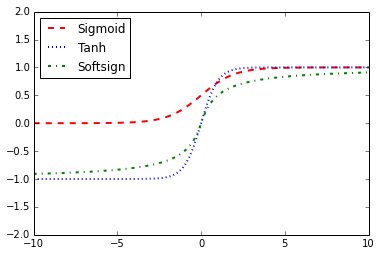
\includegraphics[width=\textwidth]{images/d2167d3b-96f9-46d1-87c4-79d0839b3745.png}
        \caption{Sigmoid, hyperbolic tangent, and softsign act func}
    \end{subfigure}
    \qquad
    ~ %add desired spacing between images, e. g. ~, \quad, \qquad, \hfill etc.
      %(or a blank line to force the subfigure onto a new line)
    \begin{subfigure}[b]{0.4\textwidth}
        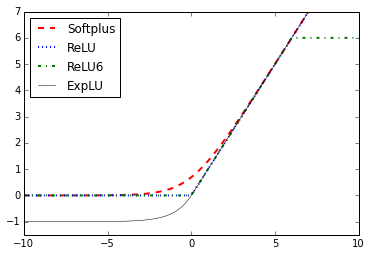
\includegraphics[width=\textwidth]{images/2a1256eb-1993-4e62-a561-48577ebcfec2.png}
        \caption{Softplus, ReLU, ReLU6, and exponential LU}
    \end{subfigure}
    \caption{Some Act Funcs}
\end{figure}


\begin{enumerate}
\item The rectified linear unit, known as ReLU, is the most common and basic way to introduce non-linearity into neural networks. This function is just called max(0,x). It is continuous, but not smooth.

\item To cap the linearly increasing part of the preceding ReLU activation function. Do this by nesting the max(0,x) function into a min() function, called the ReLU6 function.

It is computationally faster, and does not suffer from vanishing (infinitesimally near zero) or exploding values.

\item Sigmoid, most common continuous and smooth activation function. Not used very often because of its tendency to zero-out the backpropagation terms during training.

\item Softplus function, is a smooth version of the ReLU function.
\end{enumerate}



Some TensorFlow resources:
\begin{itemize}
\item A public Docker container that is kept current by TensorFlow is available on Dockerhub at \url{https://hub.docker.com/r/tensorflow/tensorflow/}

\item \textbf{[DO NOT MISS THIS]} TensorFlow has also made a site where you can visually explore training a neural network while changing the parameters and datasets. Visit \url{http://playground.tensorflow.org/} to explore how different settings affect the training of neural networks.


\end{itemize}


\ChapterCMD{2}{The TensorFlow Way}{Roderick Karlemstrand}{11 May 2019}

This chapter will cover:

\begin{itemize}
\item Operations in a computational graph
\item Layering nested operations
\item Working with multiple layers
\item Implementing loss functions
\item Implementing backpropagation
\item Working with batch and stochastic training
\item Combining everything together
\item Evaluating models
\end{itemize}

\section{Working with multiple layers}
About how to best connect various layers, including custom layers. The data we will generate and use will be representative of small random images.

The first layer we will explore is called a \textbf{moving window}. We will perform a small moving window average across a 2D image and then the second layer will be a custom operation layer.

In this section, we will see that the computational graph can get large and hard to look at. To address this, we will also introduce ways to name operations and create scopes for layers.


\begin{enumerate}
  \item Create our sample 2D image, but we use four dimensions: image number, height, width, and channel, and to make it one image with one channel, we set two of the dimensions to 1, as follows:
  \begin{lstlisting}
  x_shape = [1, 4, 4, 1]
  x_val = np.random.uniform(size=x_shape)
  \end{lstlisting}

  \item Create the placeholder in our graph where we can feed in the sample image
  \begin{lstlisting}
  x_data = tf.placeholder(tf.float32, shape=x_shape)
  \end{lstlisting}

  \item Moving window average across the 4 x 4 image, built-in function convolutes a constant across a window of the shape 2 x 2.

  The function we will use is conv2d(); this function is quite commonly used in image processing and in TensorFlow. This function takes a piecewise product of the window and a filter we specify. We must also specify a stride for the moving window in both directions. Here, we will compute four moving window averages: the upper-left, upper-right,lower-left, and lower-right four pixels. We do this by creating a 2 x 2 window and having strides of length 2 in each direction. To take the average, we will convolute the 2 x 2 window with a constant of 0.25, as follows:
  \begin{lstlisting}
  my_filter = tf.constant(0.25, shape=[2, 2, 1, 1])
  my_strides = [1, 2, 2, 1]
  mov_avg_layer= tf.nn.conv2d(x_data, my_filter, my_strides,
                              padding='SAME',
                              name='Moving_Avg_Window')
  \end{lstlisting}

  \item Define a custom layer that will operate on the 2 x 2 output of the moving window average. The custom function will first multiply the input by another 2 x 2 matrix tensor, and then add 1 to each entry.

  After this, we take the sigmoid of each element and return the 2 x 2 matrix.

  Since matrix multiplication only operates on two-dimensional matrices, we need to drop the extra dimensions of our image that are of size 1. TensorFlow can do this with the built-in squeeze() function. Here, we define the new layer:
  \begin{lstlisting}
  def custom_layer(input_matrix):
      input_matrix_sqeezed = tf.squeeze(input_matrix)
      A = tf.constant([[1., 2.], [-1., 3.]])
      b = tf.constant(1., shape=[2, 2])
      temp1 = tf.matmul(A, input_matrix_sqeezed)
      temp = tf.add(temp1, b) # Ax + b
      return tf.sigmoid(temp)
  \end{lstlisting}

  \item Place the new layer on the graph. We will do this with a named scope so that it is identifiable and collapsible/expandable on the computational graph in Tensorboard.
  \begin{lstlisting}
  with tf.name_scope('Custom_Layer') as scope:
      custom_layer1 = custom_layer(mov_avg_layer)
  \end{lstlisting}

  \item Now, we just feed in the 4 x 4 image to replace the placeholder and tell TensorFlow to run the graph, as follows:
  \begin{lstlisting}
  print(sess.run(custom_layer1, feed_dict={x_data: x_val}))
  [[ 0.91914582 0.96025133]
   [ 0.87262219  0.9469803 ]]
  \end{lstlisting}

\end{enumerate}

\begin{figure}[H]
  \centering
  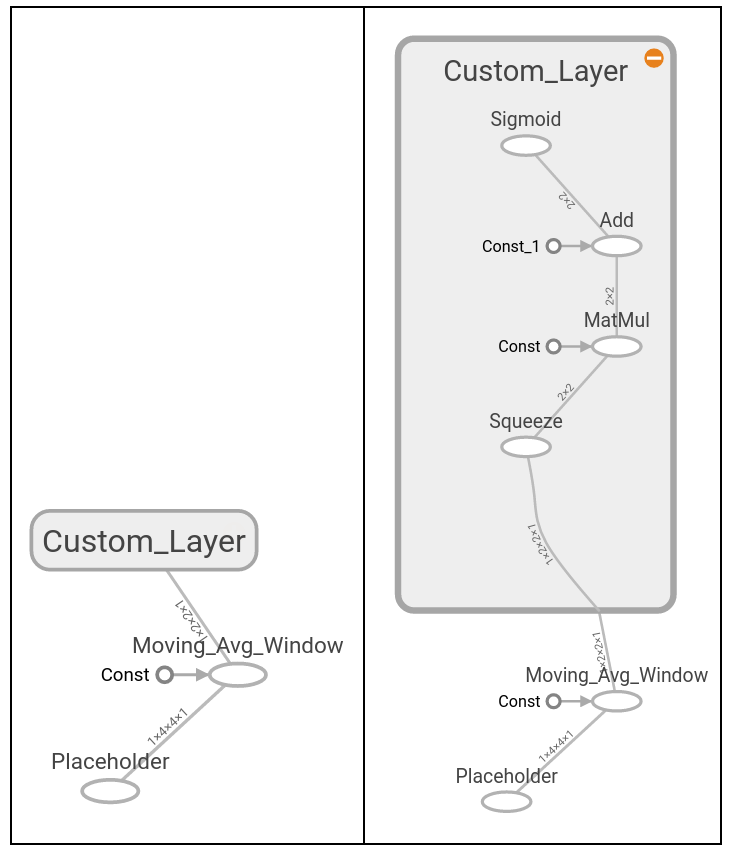
\includegraphics[width=0.8 \linewidth]{images/03_Multiple_Layers.png}
  \caption{Computational graph with two layers}
\end{figure}

\end{document}
